% ============================================================
% 讲义 — 人教版高中数学必修第一册 第5章 三角函数
% 编译命令：xelatex -interaction=nonstopmode 高一必修1_第5章_三角函数.tex
% ============================================================
\documentclass[12pt, a4paper]{ctexart}
\usepackage[margin=2.2cm]{geometry}
\usepackage{amsmath, amssymb}
\usepackage{enumitem}
\usepackage{tcolorbox}
\usepackage{booktabs}
\usepackage{array}
\usepackage{fancyhdr}
\usepackage{xcolor}
\usepackage{tikz}
\usepackage{hyperref}
\usepackage{graphicx}
\usepackage{multirow}
\usepackage{pgfplots}
\pgfplotsset{compat=1.18}

% 颜色定义
\definecolor{mainblue}{RGB}{41, 98, 168}
\definecolor{lightblue}{RGB}{230, 240, 255}
\definecolor{tipgreen}{RGB}{34, 139, 87}
\definecolor{lightgreen}{RGB}{235, 250, 240}
\definecolor{warnred}{RGB}{200, 50, 50}
\definecolor{lightred}{RGB}{255, 240, 240}
\definecolor{examorange}{RGB}{210, 120, 20}
\definecolor{lightorange}{RGB}{255, 248, 235}
\definecolor{apppurple}{RGB}{120, 60, 170}
\definecolor{lightpurple}{RGB}{245, 238, 255}

% 页眉页脚
\pagestyle{fancy}
\fancyhf{}
\fancyhead[L]{\small\textcolor{mainblue}{\textbf{人教版高中必修第一册 · 第5章}}}
\fancyhead[R]{\small\textcolor{mainblue}{三角函数讲义}}
\fancyfoot[C]{\small —\ \thepage\ —}
\renewcommand{\headrulewidth}{0.6pt}
\renewcommand{\headrule}{\hbox to\headwidth{\color{mainblue}\leaders\hrule height \headrulewidth\hfill}}
\renewcommand{\footrulewidth}{0pt}

% tcolorbox 样式
\newtcolorbox{knowledgebox}[1][]{%
  colback=lightblue, colframe=mainblue,
  fonttitle=\bfseries\large, title=#1,
  arc=3mm, boxrule=0.8pt,
  left=8pt, right=8pt, top=6pt, bottom=6pt
}

\newtcolorbox{tipbox}[1][]{%
  colback=lightgreen, colframe=tipgreen,
  fonttitle=\bfseries, title=#1,
  arc=2mm, boxrule=0.6pt,
  left=6pt, right=6pt, top=4pt, bottom=4pt
}

\newtcolorbox{warnbox}[1][]{%
  colback=lightred, colframe=warnred,
  fonttitle=\bfseries, title=#1,
  arc=2mm, boxrule=0.6pt,
  left=6pt, right=6pt, top=4pt, bottom=4pt
}

\newtcolorbox{examplebox}[1][]{%
  colback=lightorange, colframe=examorange,
  fonttitle=\bfseries, title=#1,
  arc=3mm, boxrule=0.8pt,
  left=8pt, right=8pt, top=6pt, bottom=6pt
}

\newtcolorbox{appbox}[1][]{%
  colback=lightpurple, colframe=apppurple,
  fonttitle=\bfseries, title=#1,
  arc=3mm, boxrule=0.8pt,
  left=8pt, right=8pt, top=6pt, bottom=6pt
}

\setCJKmainfont{Hiragino Sans GB}
\setCJKsansfont{Heiti SC}

\begin{document}

% ============ 标题页 ============
\begin{center}
{\Huge\bfseries\textcolor{mainblue}{第5章\quad 三角函数}}\\[12pt]
{\Large\textcolor{gray}{讲\quad 义}}\\[8pt]
\rule{0.6\textwidth}{1pt}\\[8pt]
{\normalsize 适用：人教版\quad 高中必修第一册\quad |\quad 课时：约12课时}
\end{center}
\vspace{10pt}

% ============================================================
% 第一部分：知识点讲解
% ============================================================
\section*{\textcolor{mainblue}{一、知识点讲解}}

% ---------- 5.1 任意角 ----------
\subsection*{5.1\quad 任意角的概念}

\begin{knowledgebox}[什么是"角"？]
在初中，我们知道角是从一点出发的两条射线所组成的图形。但在高中，我们需要把角的概念推广。

\medskip
\textbf{定义：}一条射线从一个位置出发，绕着它的端点旋转到另一个位置，就形成了一个角。
\begin{itemize}[leftmargin=2em]
  \item \textbf{正角：}按\textbf{逆时针}方向旋转形成的角。
  \item \textbf{负角：}按\textbf{顺时针}方向旋转形成的角。
  \item \textbf{零角：}一条射线没有做任何旋转，即旋转了$0^\circ$。
\end{itemize}
\end{knowledgebox}

\begin{tipbox}[理解要点]
角的正负只表示旋转方向，不代表大小。例如，$-30^\circ$和$30^\circ$的终边不同，但它们的绝对值相同。
\end{tipbox}

\begin{knowledgebox}[象限角与轴线角]
把角的顶点放在坐标原点，始边与$x$轴的正半轴重合，那么终边落在第几象限，就叫第几象限角。

\medskip
\begin{tabular}{ll}
\toprule
\textbf{终边位置} & \textbf{角的范围} \\
\midrule
第一象限 & $k\cdot360^\circ<\alpha<k\cdot360^\circ+90^\circ$\\
第二象限 & $k\cdot360^\circ+90^\circ<\alpha<k\cdot360^\circ+180^\circ$\\
第三象限 & $k\cdot360^\circ+180^\circ<\alpha<k\cdot360^\circ+270^\circ$\\
第四象限 & $k\cdot360^\circ+270^\circ<\alpha<k\cdot360^\circ+360^\circ$\\
\bottomrule
\end{tabular}

\medskip
其中$k\in\mathbb{Z}$。终边落在坐标轴上的角叫做\textbf{轴线角}。
\end{knowledgebox}

\begin{warnbox}[易错提醒]
"第一象限角"不等于"锐角"！例如$390^\circ$是第一象限角，但不是锐角（锐角是$0^\circ\sim90^\circ$）。同样，$-300^\circ$也是第一象限角。第一象限角是一个无限的集合。
\end{warnbox}

\begin{knowledgebox}[终边相同的角]
与角$\alpha$终边相同的角的集合为：
\[
  \{\beta\mid\beta=\alpha+k\cdot360^\circ,\;k\in\mathbb{Z}\}
\]
\end{knowledgebox}

% ---------- 5.2 弧度制 ----------
\subsection*{5.2\quad 弧度制}

\begin{knowledgebox}[弧度的定义]
\textbf{弧度制}是另一种度量角的方法。

\medskip
\textbf{定义：}长度等于半径的弧所对的圆心角叫做\textbf{1弧度}的角，记作$1\,\text{rad}$。

\medskip
\textbf{关键换算：}
\[
  \boxed{\pi\,\text{rad}=180^\circ}
\]
由此可得：
\[
  1\,\text{rad}=\frac{180^\circ}{\pi}\approx57.30^\circ, \qquad
  1^\circ=\frac{\pi}{180}\,\text{rad}\approx0.01745\,\text{rad}
\]
\end{knowledgebox}

\begin{tipbox}[常见角度的弧度与角度对照]
\begin{center}
\begin{tabular}{ccccccccccc}
\toprule
角度 & $0^\circ$ & $30^\circ$ & $45^\circ$ & $60^\circ$ & $90^\circ$ & $120^\circ$ & $135^\circ$ & $150^\circ$ & $180^\circ$ & $360^\circ$ \\
\midrule
弧度 & $0$ & $\dfrac{\pi}{6}$ & $\dfrac{\pi}{4}$ & $\dfrac{\pi}{3}$ & $\dfrac{\pi}{2}$ & $\dfrac{2\pi}{3}$ & $\dfrac{3\pi}{4}$ & $\dfrac{5\pi}{6}$ & $\pi$ & $2\pi$ \\
\bottomrule
\end{tabular}
\end{center}
务必牢记这张表，后面做题时会频繁使用。
\end{tipbox}

\begin{knowledgebox}[弧长公式与扇形面积]
设圆的半径为$r$，圆心角为$\alpha$（弧度），弧长为$l$，扇形面积为$S$，则：

\medskip
\textbf{弧长公式：}
\[
  \boxed{l=|\alpha|\,r}
\]

\textbf{扇形面积公式：}
\[
  \boxed{S=\frac{1}{2}lr=\frac{1}{2}|\alpha|\,r^2}
\]

这两个公式的记忆方法：弧度制下的公式比角度制下更简洁，这就是引入弧度制的好处。
\end{knowledgebox}

% ---------- 5.3 任意角的三角函数 ----------
\subsection*{5.3\quad 任意角的三角函数}

\begin{knowledgebox}[单位圆上的三角函数定义]
在直角坐标系中，以原点为圆心、$1$为半径作圆（\textbf{单位圆}）。设角$\alpha$的终边与单位圆的交点为$P(x,y)$，则：

\[
  \boxed{\cos\alpha=x,\quad \sin\alpha=y,\quad \tan\alpha=\frac{y}{x}\;(x\neq0)}
\]

\begin{center}
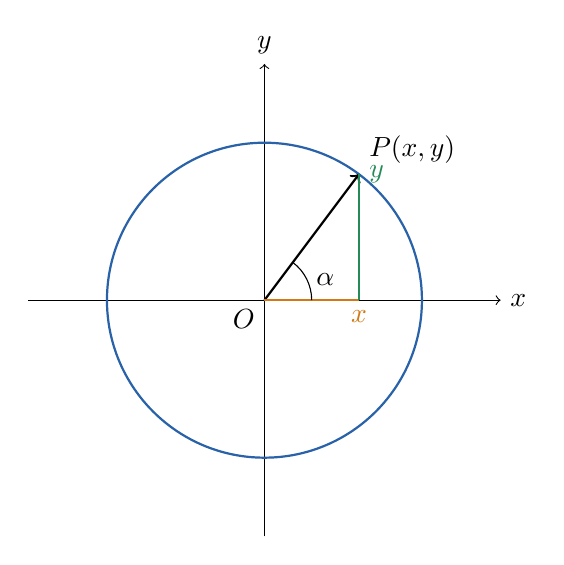
\begin{tikzpicture}[scale=2]
  \draw[->] (-1.5,0) -- (1.5,0) node[right]{$x$};
  \draw[->] (0,-1.5) -- (0,1.5) node[above]{$y$};
  \draw[thick, mainblue] (0,0) circle(1);
  \coordinate (O) at (0,0);
  \coordinate (P) at (0.6,0.8);
  \draw[thick, ->] (O) -- (P) node[above right]{$P(x,y)$};
  \draw[thick, examorange] (O) -- (P |- O) node[below]{$x$};
  \draw[thick, tipgreen] (P |- O) -- (P) node[right]{$y$};
  \draw (0.3,0) arc(0:53.13:0.3) node[midway, right]{$\alpha$};
  \node[below left] at (0,0) {$O$};
\end{tikzpicture}
\end{center}

\medskip
\textbf{几何意义：}
\begin{itemize}[leftmargin=2em]
  \item $\cos\alpha$等于终边与单位圆交点的\textbf{横坐标}。
  \item $\sin\alpha$等于终边与单位圆交点的\textbf{纵坐标}。
  \item $\tan\alpha$可以理解为终边（或其反向延长线）与直线$x=1$交点的纵坐标。
\end{itemize}
\end{knowledgebox}

\begin{knowledgebox}[三角函数的符号]
根据终边所在象限确定三角函数的正负号：

\medskip
\begin{center}
\begin{tabular}{cccc}
\toprule
 & 第一象限 & 第二象限 & 第三象限 & 第四象限 \\
\midrule
$\sin\alpha$ & $+$ & $+$ & $-$ & $-$ \\
$\cos\alpha$ & $+$ & $-$ & $-$ & $+$ \\
$\tan\alpha$ & $+$ & $-$ & $+$ & $-$ \\
\bottomrule
\end{tabular}
\end{center}

\medskip
\textbf{口诀：}一全正，二正弦，三正切，四余弦。（意思是该象限中哪个三角函数为正）
\end{knowledgebox}

\begin{knowledgebox}[特殊角的三角函数值]
\begin{center}
\begin{tabular}{cccccc}
\toprule
$\alpha$ & $0$ & $\dfrac{\pi}{6}$ & $\dfrac{\pi}{4}$ & $\dfrac{\pi}{3}$ & $\dfrac{\pi}{2}$ \\[6pt]
\midrule
$\sin\alpha$ & $0$ & $\dfrac{1}{2}$ & $\dfrac{\sqrt{2}}{2}$ & $\dfrac{\sqrt{3}}{2}$ & $1$ \\[6pt]
$\cos\alpha$ & $1$ & $\dfrac{\sqrt{3}}{2}$ & $\dfrac{\sqrt{2}}{2}$ & $\dfrac{1}{2}$ & $0$ \\[6pt]
$\tan\alpha$ & $0$ & $\dfrac{\sqrt{3}}{3}$ & $1$ & $\sqrt{3}$ & 不存在 \\
\bottomrule
\end{tabular}
\end{center}
\end{knowledgebox}

% ---------- 5.4 同角三角函数基本关系 ----------
\subsection*{5.4\quad 同角三角函数基本关系}

\begin{knowledgebox}[两个基本关系式]
设$\alpha$是任意角，则：

\medskip
\textbf{（1）平方关系：}
\[
  \boxed{\sin^2\alpha+\cos^2\alpha=1}
\]

\textbf{（2）商数关系：}
\[
  \boxed{\tan\alpha=\frac{\sin\alpha}{\cos\alpha}\quad(\cos\alpha\neq0)}
\]
\end{knowledgebox}

\begin{warnbox}[易错提醒]
\begin{enumerate}[leftmargin=2em]
  \item $\sin^2\alpha$表示$(\sin\alpha)^2$，不要写成$\sin\alpha^2$。
  \item 由$\sin^2\alpha+\cos^2\alpha=1$可以变形为$\sin^2\alpha=1-\cos^2\alpha$和$\cos^2\alpha=1-\sin^2\alpha$。
  \item 由$\tan\alpha=\dfrac{\sin\alpha}{\cos\alpha}$可以推出$\sin\alpha=\tan\alpha\cdot\cos\alpha$。
\end{enumerate}
\end{warnbox}

% ---------- 5.5 诱导公式 ----------
\subsection*{5.5\quad 诱导公式}

\begin{knowledgebox}[诱导公式（六组）]
诱导公式的作用：将任意角的三角函数转化为锐角三角函数。

\medskip
\textbf{公式一（终边相同的角）：}
\[
  \sin(\alpha+2k\pi)=\sin\alpha,\quad \cos(\alpha+2k\pi)=\cos\alpha,\quad \tan(\alpha+2k\pi)=\tan\alpha
\]

\textbf{公式二：}
\[
  \sin(\pi+\alpha)=-\sin\alpha,\quad \cos(\pi+\alpha)=-\cos\alpha,\quad \tan(\pi+\alpha)=\tan\alpha
\]

\textbf{公式三：}
\[
  \sin(-\alpha)=-\sin\alpha,\quad \cos(-\alpha)=\cos\alpha,\quad \tan(-\alpha)=-\tan\alpha
\]

\textbf{公式四：}
\[
  \sin(\pi-\alpha)=\sin\alpha,\quad \cos(\pi-\alpha)=-\cos\alpha,\quad \tan(\pi-\alpha)=-\tan\alpha
\]

\textbf{公式五：}
\[
  \sin\!\left(\frac{\pi}{2}-\alpha\right)=\cos\alpha,\quad \cos\!\left(\frac{\pi}{2}-\alpha\right)=\sin\alpha
\]

\textbf{公式六：}
\[
  \sin\!\left(\frac{\pi}{2}+\alpha\right)=\cos\alpha,\quad \cos\!\left(\frac{\pi}{2}+\alpha\right)=-\sin\alpha
\]
\end{knowledgebox}

\begin{tipbox}[口诀：奇变偶不变，符号看象限]
\textbf{解释：}
\begin{itemize}[leftmargin=2em]
  \item \textbf{奇变偶不变：}$\dfrac{\pi}{2}$的\textbf{奇数倍}$+\alpha$（如$\dfrac{\pi}{2}\pm\alpha$）时，函数名要变（$\sin\leftrightarrow\cos$）；$\dfrac{\pi}{2}$的\textbf{偶数倍}$+\alpha$（如$\pi\pm\alpha$，$2\pi+\alpha$）时，函数名不变。
  \item \textbf{符号看象限：}把$\alpha$看成锐角，看变换后的角在第几象限，确定正负号。
\end{itemize}

\medskip
\textbf{举例：}$\sin\!\left(\dfrac{3\pi}{2}+\alpha\right)$

$\dfrac{3\pi}{2}=\dfrac{\pi}{2}\times3$，是奇数倍，所以函数名变：$\sin\to\cos$。

把$\alpha$看作锐角，$\dfrac{3\pi}{2}+\alpha$在第四象限，$\sin$为负，所以：
\[
  \sin\!\left(\frac{3\pi}{2}+\alpha\right)=-\cos\alpha
\]
\end{tipbox}

% ---------- 5.6 三角函数的图象与性质 ----------
\subsection*{5.6\quad 三角函数的图象与性质}

\begin{knowledgebox}[$y=\sin x$的图象与性质]

\begin{center}
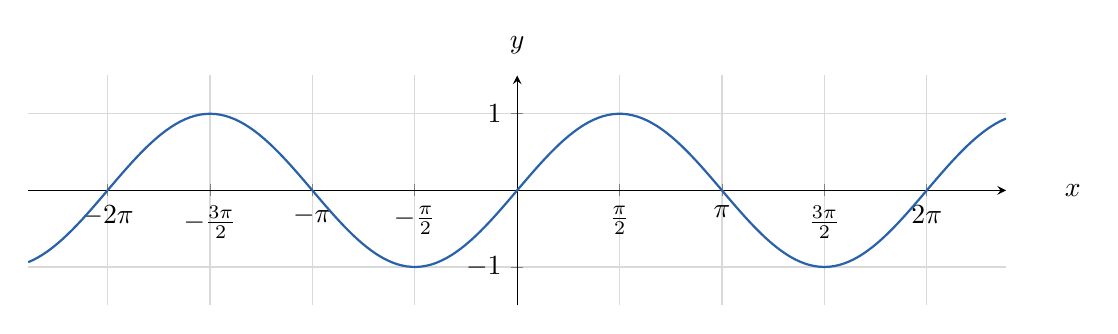
\begin{tikzpicture}
\begin{axis}[
  width=14cm, height=4.5cm,
  axis lines=middle,
  xlabel={$x$}, ylabel={$y$},
  xmin=-7.5, xmax=7.5,
  ymin=-1.5, ymax=1.5,
  xtick={-6.283, -4.712, -3.1416, -1.5708, 0, 1.5708, 3.1416, 4.712, 6.283},
  xticklabels={$-2\pi$, {$-\frac{3\pi}{2}$}, {$-\pi$}, {$-\frac{\pi}{2}$}, $0$, {$\frac{\pi}{2}$}, {$\pi$}, {$\frac{3\pi}{2}$}, {$2\pi$}},
  ytick={-1, 1},
  yticklabels={$-1$, $1$},
  grid=both,
  grid style={gray!30},
  every axis x label/.style={at={(ticklabel* cs:1.05)}, anchor=west},
  every axis y label/.style={at={(ticklabel* cs:1.05)}, anchor=south},
  samples=200,
]
\addplot[thick, mainblue, domain=-7.5:7.5]{sin(deg(x))};
\end{axis}
\end{tikzpicture}
\end{center}

\medskip
\begin{tabular}{ll}
\toprule
\textbf{性质} & \textbf{内容} \\
\midrule
定义域 & $\mathbb{R}$（全体实数） \\
值域 & $[-1,1]$ \\
周期 & $T=2\pi$ \\
奇偶性 & $\sin(-x)=-\sin x$，是\textbf{奇函数} \\
单调递增区间 & $\left[-\dfrac{\pi}{2}+2k\pi,\;\dfrac{\pi}{2}+2k\pi\right],\;k\in\mathbb{Z}$ \\
单调递减区间 & $\left[\dfrac{\pi}{2}+2k\pi,\;\dfrac{3\pi}{2}+2k\pi\right],\;k\in\mathbb{Z}$ \\
最大值 & $y_{\max}=1$，当$x=\dfrac{\pi}{2}+2k\pi$时取到 \\
最小值 & $y_{\min}=-1$，当$x=-\dfrac{\pi}{2}+2k\pi$时取到 \\
\bottomrule
\end{tabular}
\end{knowledgebox}

\begin{knowledgebox}[$y=\cos x$的图象与性质]

\begin{center}
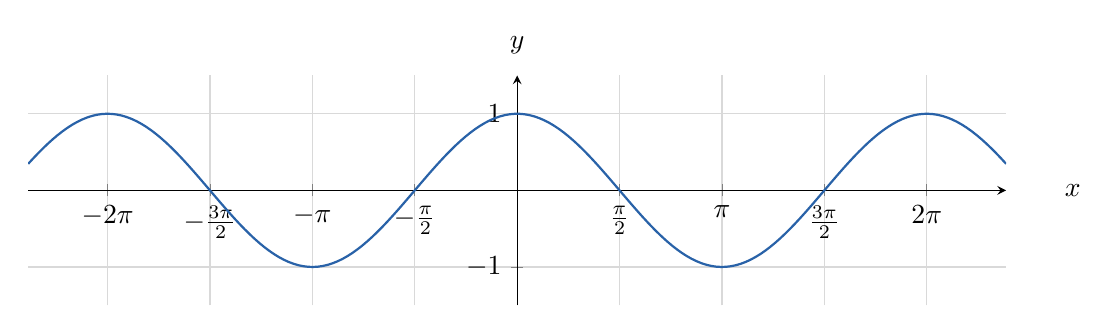
\begin{tikzpicture}
\begin{axis}[
  width=14cm, height=4.5cm,
  axis lines=middle,
  xlabel={$x$}, ylabel={$y$},
  xmin=-7.5, xmax=7.5,
  ymin=-1.5, ymax=1.5,
  xtick={-6.283, -4.712, -3.1416, -1.5708, 0, 1.5708, 3.1416, 4.712, 6.283},
  xticklabels={$-2\pi$, {$-\frac{3\pi}{2}$}, {$-\pi$}, {$-\frac{\pi}{2}$}, $0$, {$\frac{\pi}{2}$}, {$\pi$}, {$\frac{3\pi}{2}$}, {$2\pi$}},
  ytick={-1, 1},
  yticklabels={$-1$, $1$},
  grid=both,
  grid style={gray!30},
  every axis x label/.style={at={(ticklabel* cs:1.05)}, anchor=west},
  every axis y label/.style={at={(ticklabel* cs:1.05)}, anchor=south},
  samples=200,
]
\addplot[thick, mainblue, domain=-7.5:7.5]{cos(deg(x))};
\end{axis}
\end{tikzpicture}
\end{center}

\medskip
\begin{tabular}{ll}
\toprule
\textbf{性质} & \textbf{内容} \\
\midrule
定义域 & $\mathbb{R}$ \\
值域 & $[-1,1]$ \\
周期 & $T=2\pi$ \\
奇偶性 & $\cos(-x)=\cos x$，是\textbf{偶函数} \\
单调递增区间 & $[-\pi+2k\pi,\;2k\pi],\;k\in\mathbb{Z}$ \\
单调递减区间 & $[2k\pi,\;\pi+2k\pi],\;k\in\mathbb{Z}$ \\
最大值 & $y_{\max}=1$，当$x=2k\pi$时取到 \\
最小值 & $y_{\min}=-1$，当$x=\pi+2k\pi$时取到 \\
\bottomrule
\end{tabular}
\end{knowledgebox}

\begin{knowledgebox}[$y=\tan x$的图象与性质]

\begin{center}
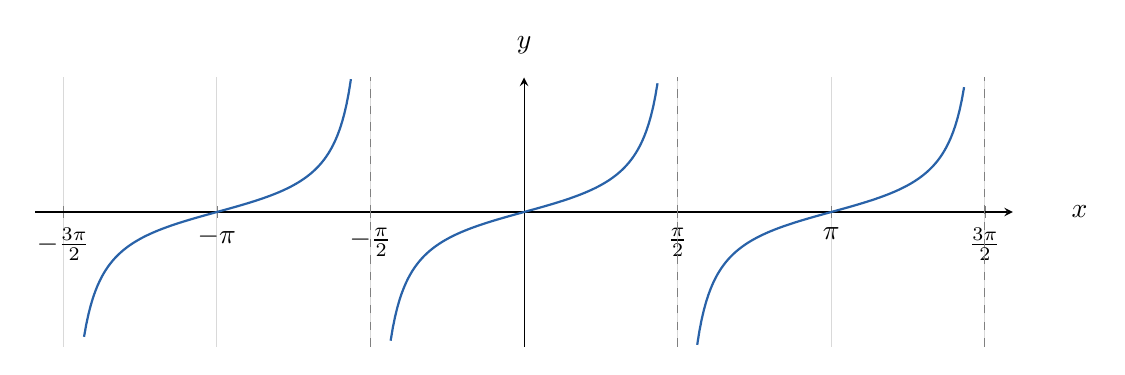
\begin{tikzpicture}
\begin{axis}[
  width=14cm, height=5cm,
  axis lines=middle,
  xlabel={$x$}, ylabel={$y$},
  xmin=-5, xmax=5,
  ymin=-5, ymax=5,
  xtick={-4.712, -3.1416, -1.5708, 0, 1.5708, 3.1416, 4.712},
  xticklabels={$-\frac{3\pi}{2}$, {$-\pi$}, {$-\frac{\pi}{2}$}, $0$, {$\frac{\pi}{2}$}, {$\pi$}, {$\frac{3\pi}{2}$}},
  ytick=\empty,
  grid=both,
  grid style={gray!30},
  every axis x label/.style={at={(ticklabel* cs:1.05)}, anchor=west},
  every axis y label/.style={at={(ticklabel* cs:1.05)}, anchor=south},
  samples=400,
  restrict y to domain=-5:5,
]
\addplot[thick, mainblue, domain=-4.5:4.5]{tan(deg(x))};
\draw[dashed, gray] (axis cs:-1.5708,-5) -- (axis cs:-1.5708,5);
\draw[dashed, gray] (axis cs:1.5708,-5) -- (axis cs:1.5708,5);
\draw[dashed, gray] (axis cs:4.712,-5) -- (axis cs:4.712,5);
\end{axis}
\end{tikzpicture}
\end{center}

\medskip
\begin{tabular}{ll}
\toprule
\textbf{性质} & \textbf{内容} \\
\midrule
定义域 & $\left\{x\;\Big|\;x\neq\dfrac{\pi}{2}+k\pi,\;k\in\mathbb{Z}\right\}$ \\
值域 & $\mathbb{R}$ \\
周期 & $T=\pi$ \\
奇偶性 & $\tan(-x)=-\tan x$，是\textbf{奇函数} \\
单调递增区间 & $\left(-\dfrac{\pi}{2}+k\pi,\;\dfrac{\pi}{2}+k\pi\right),\;k\in\mathbb{Z}$ \\
\bottomrule
\end{tabular}

\medskip
\begin{warnbox}[注意]
$\tan x$在整个定义域上不是连续函数。它在每个开区间$\left(-\dfrac{\pi}{2}+k\pi,\;\dfrac{\pi}{2}+k\pi\right)$上是单调递增的，但不能说"$\tan x$在整个定义域上单调递增"。
\end{warnbox}
\end{knowledgebox}

% ---------- 5.7 正弦型函数 ----------
\subsection*{5.7\quad 函数$y=A\sin(\omega x+\varphi)$的图象与性质}

\begin{knowledgebox}[正弦型函数的三个参数]
函数$y=A\sin(\omega x+\varphi)$（其中$A>0$，$\omega>0$）中：

\begin{itemize}[leftmargin=2em]
  \item $A$：\textbf{振幅}，图象上最高点的纵坐标，值域为$[-A,A]$。
  \item $\omega$：\textbf{角频率}，与周期的关系为$T=\dfrac{2\pi}{\omega}$。
  \item $\varphi$：\textbf{初相}，影响图象的左右平移。
\end{itemize}
\end{knowledgebox}

\begin{knowledgebox}[图象变换（重点！）]
由$y=\sin x$的图象得到$y=A\sin(\omega x+\varphi)$的图象有两种变换路径：

\medskip
\textbf{路径一（先平移后伸缩，推荐）：}

\begin{enumerate}[leftmargin=2em]
  \item \textbf{左右平移：}$y=\sin x\;\xrightarrow{\text{向左平移}\varphi\text{个单位}}\;y=\sin(x+\varphi)$
  \item \textbf{横坐标伸缩：}$y=\sin(x+\varphi)\;\xrightarrow{\text{横坐标缩短为}\frac{1}{\omega}}\;y=\sin(\omega x+\varphi)$
  \item \textbf{纵坐标伸缩：}$y=\sin(\omega x+\varphi)\;\xrightarrow{\text{纵坐标伸长为}A\text{倍}}\;y=A\sin(\omega x+\varphi)$
\end{enumerate}

\textbf{路径二（先伸缩后平移）：}

\begin{enumerate}[leftmargin=2em]
  \item \textbf{横坐标伸缩：}$y=\sin x\;\xrightarrow{\text{横坐标缩短为}\frac{1}{\omega}}\;y=\sin\omega x$
  \item \textbf{左右平移：}$y=\sin\omega x\;\xrightarrow{\text{向左平移}\frac{\varphi}{\omega}\text{个单位}}\;y=\sin(\omega x+\varphi)$
  \item \textbf{纵坐标伸缩：}同上。
\end{enumerate}

\medskip
\begin{warnbox}[易错提醒]
路径二中，第二步是向左平移$\dfrac{\varphi}{\omega}$个单位（不是$\varphi$个单位！），因为此时自变量$x$的系数是$\omega$。
\end{warnbox}
\end{knowledgebox}

\begin{knowledgebox}[正弦型函数的性质]
对于$y=A\sin(\omega x+\varphi)$（$A>0$，$\omega>0$）：

\begin{itemize}[leftmargin=2em]
  \item \textbf{周期：}$T=\dfrac{2\pi}{\omega}$
  \item \textbf{最大值：}$A$，\textbf{最小值：}$-A$
  \item \textbf{单调递增区间：}令$-\dfrac{\pi}{2}+2k\pi\leqslant\omega x+\varphi\leqslant\dfrac{\pi}{2}+2k\pi$，解出$x$的范围。
  \item \textbf{单调递减区间：}令$\dfrac{\pi}{2}+2k\pi\leqslant\omega x+\varphi\leqslant\dfrac{3\pi}{2}+2k\pi$，解出$x$的范围。
\end{itemize}

\medskip
\textbf{求单调区间的方法：}把$\omega x+\varphi$看作一个整体$t$，先写出$\sin t$的单调区间（与$y=\sin x$的相同），再通过$t=\omega x+\varphi$解出$x$。
\end{knowledgebox}

% ============================================================
% 第二部分：例题精讲
% ============================================================
\newpage
\section*{\textcolor{examorange}{二、例题精讲}}

% ---- 例题1 ----
\begin{examplebox}[【例题1】角度与弧度的互化]
将下列各角进行角度与弧度的互化：

\textbf{(1)} $225^\circ=$\underline{\qquad}$\,\text{rad}$\qquad\textbf{(2)} $\dfrac{5\pi}{12}=$\underline{\qquad}^\circ$

\textbf{(3)} $-150^\circ=$\underline{\qquad}$\,\text{rad}$
\end{examplebox}

\textbf{解：}

\textbf{(1)} 利用公式$1^\circ=\dfrac{\pi}{180}\,\text{rad}$：
\[
  225^\circ=225\times\frac{\pi}{180}=\frac{225\pi}{180}=\frac{5\pi}{4}\,\text{rad}
\]

\textbf{(2)} 利用公式$1\,\text{rad}=\dfrac{180^\circ}{\pi}$：
\[
  \frac{5\pi}{12}=\frac{5\pi}{12}\times\frac{180^\circ}{\pi}=\frac{5\times180^\circ}{12}=75^\circ
\]

\textbf{(3)} $-150^\circ=-150\times\dfrac{\pi}{180}=-\dfrac{5\pi}{6}\,\text{rad}$

\begin{tipbox}[方法总结]
互化的核心公式就两个：$\pi\,\text{rad}=180^\circ$。做题时先把$\pi$和$180^\circ$互换，再约分即可。
\end{tipbox}

% ---- 例题2 ----
\begin{examplebox}[【例题2】扇形的弧长与面积]
已知扇形的圆心角为$120^\circ$，半径为$6\,\text{cm}$，求扇形的弧长和面积。
\end{examplebox}

\textbf{解：}

首先将$120^\circ$转化为弧度：
\[
  120^\circ=120\times\frac{\pi}{180}=\frac{2\pi}{3}\,\text{rad}
\]

弧长：
\[
  l=|\alpha|\,r=\frac{2\pi}{3}\times6=4\pi\,(\text{cm})
\]

面积：
\[
  S=\frac{1}{2}lr=\frac{1}{2}\times4\pi\times6=12\pi\,(\text{cm}^2)
\]

\begin{tipbox}[方法总结]
用弧度制的公式更简洁：$l=|\alpha|r$，$S=\frac{1}{2}lr$。注意先将角度化为弧度再代入。
\end{tipbox}

% ---- 例题3 ----
\begin{examplebox}[【例题3】判断角所在的象限]
判断下列各角是第几象限角：

\textbf{(1)} $510^\circ$\qquad\textbf{(2)} $-\dfrac{7\pi}{4}$\qquad\textbf{(3)} $-950^\circ$
\end{examplebox}

\textbf{解：}

\textbf{(1)} $510^\circ=360^\circ+150^\circ$，终边与$150^\circ$相同，$150^\circ$在\textbf{第二象限}。

\textbf{(2)} $-\dfrac{7\pi}{4}$加上$2\pi$：$-\dfrac{7\pi}{4}+2\pi=-\dfrac{7\pi}{4}+\dfrac{8\pi}{4}=\dfrac{\pi}{4}$，终边与$\dfrac{\pi}{4}$相同，$\dfrac{\pi}{4}$在\textbf{第一象限}。

\textbf{(3)} $-950^\circ$加上$3\times360^\circ=1080^\circ$：$-950^\circ+1080^\circ=130^\circ$，终边与$130^\circ$相同，$130^\circ$在\textbf{第二象限}。

\begin{tipbox}[方法总结]
判断象限角的步骤：用加减$360^\circ$（或$2\pi$）的整数倍，将角化到$0^\circ\sim360^\circ$（或$0\sim2\pi$）的范围内，再判断。
\end{tipbox}

% ---- 例题4 ----
\begin{examplebox}[【例题4】已知三角函数值求其他三角函数值]
已知$\sin\alpha=\dfrac{3}{5}$，且$\alpha$为第二象限角，求$\cos\alpha$和$\tan\alpha$。
\end{examplebox}

\textbf{解：}

由$\sin^2\alpha+\cos^2\alpha=1$得：
\[
  \cos^2\alpha=1-\sin^2\alpha=1-\left(\frac{3}{5}\right)^2=1-\frac{9}{25}=\frac{16}{25}
\]
\[
  \cos\alpha=\pm\frac{4}{5}
\]

因为$\alpha$为第二象限角，$\cos\alpha<0$，所以$\cos\alpha=-\dfrac{4}{5}$。

\[
  \tan\alpha=\frac{\sin\alpha}{\cos\alpha}=\frac{\frac{3}{5}}{-\frac{4}{5}}=-\frac{3}{4}
\]

\begin{tipbox}[方法总结]
利用平方关系求出$\cos\alpha$后，必须根据$\alpha$所在的象限确定符号。第二象限中$\sin>0$，$\cos<0$。
\end{tipbox}

% ---- 例题5 ----
\begin{examplebox}[【例题5】利用诱导公式化简求值]
求值：$\sin\dfrac{7\pi}{6}+\cos\dfrac{5\pi}{3}-\tan\dfrac{7\pi}{4}$。
\end{examplebox}

\textbf{解：}

逐项化简：

$\sin\dfrac{7\pi}{6}=\sin\!\left(\pi+\dfrac{\pi}{6}\right)=-\sin\dfrac{\pi}{6}=-\dfrac{1}{2}$（公式二）

$\cos\dfrac{5\pi}{3}=\cos\!\left(2\pi-\dfrac{\pi}{3}\right)=\cos\dfrac{\pi}{3}=\dfrac{1}{2}$（公式一）

$\tan\dfrac{7\pi}{4}=\tan\!\left(2\pi-\dfrac{\pi}{4}\right)=\tan\!\left(-\dfrac{\pi}{4}\right)=-\tan\dfrac{\pi}{4}=-1$（公式一、公式三）

\[
  \text{原式}=-\frac{1}{2}+\frac{1}{2}-(-1)=-\frac{1}{2}+\frac{1}{2}+1=1
\]

% ---- 例题6 ----
\begin{examplebox}[【例题6】诱导公式综合化简]
化简：$\dfrac{\sin(\pi+\alpha)\cos(2\pi-\alpha)\tan(-\alpha+\pi)}{\cos(-\alpha)\sin(-\pi-\alpha)}$。
\end{examplebox}

\textbf{解：}

逐项化简（利用诱导公式）：

$\sin(\pi+\alpha)=-\sin\alpha$

$\cos(2\pi-\alpha)=\cos(-\alpha)=\cos\alpha$

$\tan(-\alpha+\pi)=\tan(\pi-\alpha)=-\tan\alpha=-\dfrac{\sin\alpha}{\cos\alpha}$

$\cos(-\alpha)=\cos\alpha$

$\sin(-\pi-\alpha)=\sin[-(\pi+\alpha)]=-\sin(\pi+\alpha)=-(-\sin\alpha)=\sin\alpha$

代入：
\[
  \text{原式}=\frac{(-\sin\alpha)\cdot\cos\alpha\cdot\left(-\dfrac{\sin\alpha}{\cos\alpha}\right)}{\cos\alpha\cdot\sin\alpha}
  =\frac{\dfrac{\sin^2\alpha\cos\alpha}{\cos\alpha}}{\cos\alpha\sin\alpha}
  =\frac{\sin^2\alpha}{\cos\alpha\sin\alpha}
  =\frac{\sin\alpha}{\cos\alpha}
  =\tan\alpha
\]

\begin{tipbox}[方法总结]
诱导公式化简的关键步骤：
\begin{enumerate}[leftmargin=2em]
  \item 先用诱导公式将每个三角函数化为$\alpha$的三角函数；
  \item 再用商数关系$\tan\alpha=\dfrac{\sin\alpha}{\cos\alpha}$统一化简。
\end{enumerate}
\end{tipbox}

% ---- 例题7 ----
\begin{examplebox}[【例题7】求正弦型函数的周期与单调区间]
求函数$y=2\sin\!\left(2x+\dfrac{\pi}{6}\right)$的周期、单调递增区间和最大值。
\end{examplebox}

\textbf{解：}

\textbf{（1）周期：}$T=\dfrac{2\pi}{\omega}=\dfrac{2\pi}{2}=\pi$

\textbf{（2）单调递增区间：}

$y=\sin t$的单调递增区间为$-\dfrac{\pi}{2}+2k\pi\leqslant t\leqslant\dfrac{\pi}{2}+2k\pi$。

令$t=2x+\dfrac{\pi}{6}$，则：
\[
  -\frac{\pi}{2}+2k\pi\leqslant 2x+\frac{\pi}{6}\leqslant\frac{\pi}{2}+2k\pi
\]

三边同时减去$\dfrac{\pi}{6}$：
\[
  -\frac{\pi}{2}-\frac{\pi}{6}+2k\pi\leqslant 2x\leqslant\frac{\pi}{2}-\frac{\pi}{6}+2k\pi
\]
\[
  -\frac{2\pi}{3}+2k\pi\leqslant 2x\leqslant\frac{\pi}{3}+2k\pi
\]

三边同时除以$2$：
\[
  \boxed{-\frac{\pi}{3}+k\pi\leqslant x\leqslant\frac{\pi}{6}+k\pi,\quad k\in\mathbb{Z}}
\]

\textbf{（3）最大值：}$y_{\max}=A=2$（当$\sin\!\left(2x+\dfrac{\pi}{6}\right)=1$时，即$2x+\dfrac{\pi}{6}=\dfrac{\pi}{2}+2k\pi$，$x=\dfrac{\pi}{6}+k\pi$时取到。）

% ---- 例题8 ----
\begin{examplebox}[【例题8】图象变换——由$y=\sin x$到$y=A\sin(\omega x+\varphi)$]
说明如何由$y=\sin x$的图象经过变换得到$y=3\sin\!\left(2x-\dfrac{\pi}{3}\right)$的图象。
\end{examplebox}

\textbf{解：}

先将函数改写为$y=3\sin\!\left(2\left(x-\dfrac{\pi}{6}\right)\right)$。

\textbf{路径一（先平移，后伸缩）：}

\begin{enumerate}[leftmargin=2em]
  \item 将$y=\sin x$的图象\textbf{向右平移}$\dfrac{\pi}{6}$个单位，得到$y=\sin\!\left(x-\dfrac{\pi}{6}\right)$。
  \item 将所得图象上所有点的\textbf{横坐标缩短为原来的}$\dfrac{1}{2}$（纵坐标不变），得到$y=\sin\!\left(2x-\dfrac{\pi}{3}\right)$。
  \item 将所得图象上所有点的\textbf{纵坐标伸长为原来的$3$倍}（横坐标不变），得到$y=3\sin\!\left(2x-\dfrac{\pi}{3}\right)$。
\end{enumerate}

\begin{warnbox}[易错提醒]
注意函数中是$2x-\dfrac{\pi}{3}$，不是$2x+\dfrac{\pi}{3}$。提取系数$2$后得到$2\left(x-\dfrac{\pi}{6}\right)$，所以是向\textbf{右}平移$\dfrac{\pi}{6}$个单位，不是向左。
\end{warnbox}

% ---- 例题9 ----
\begin{examplebox}[【例题9】由图象确定正弦型函数的解析式]
如下图所示，已知函数$y=A\sin(\omega x+\varphi)$（$A>0$，$\omega>0$，$|\varphi|<\dfrac{\pi}{2}$）的部分图象，求函数的解析式。

\begin{center}
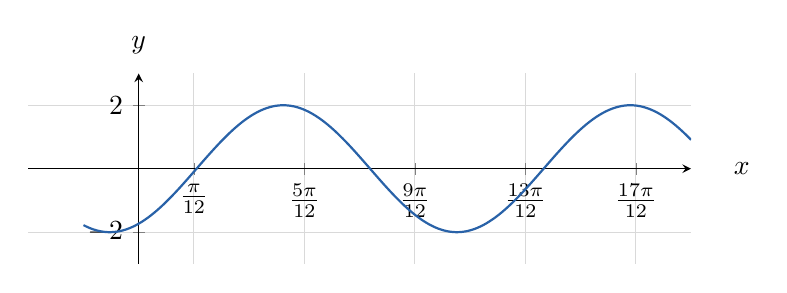
\begin{tikzpicture}
\begin{axis}[
  width=10cm, height=4cm,
  axis lines=middle,
  xlabel={$x$}, ylabel={$y$},
  xmin=-1, xmax=5,
  ymin=-3, ymax=3,
  xtick={0.5, 1.5, 2.5, 3.5, 4.5},
  xticklabels={$\frac{\pi}{12}$, {$\frac{5\pi}{12}$}, {$\frac{9\pi}{12}$}, {$\frac{13\pi}{12}$}, {$\frac{17\pi}{12}$}},
  ytick={-2, 2},
  yticklabels={$-2$, $2$},
  grid=both,
  grid style={gray!30},
  every axis x label/.style={at={(ticklabel* cs:1.05)}, anchor=west},
  every axis y label/.style={at={(ticklabel* cs:1.05)}, anchor=south},
  samples=200,
]
\addplot[thick, mainblue, domain=-0.5:5]{2*sin(deg(2*x - pi/3))};
\end{axis}
\end{tikzpicture}
\end{center}
\end{examplebox}

\textbf{解：}

\textbf{（1）求$A$：}由图象知最大值为$2$，所以$A=2$。

\textbf{（2）求$\omega$：}由图象知$T\approx\pi$（相邻两个最高点的距离约为$\pi$），所以：
\[
  T=\frac{2\pi}{\omega}=\pi\implies\omega=2
\]

\textbf{（3）求$\varphi$：}令$y=2\sin(2x+\varphi)$，由图象知当$x=\dfrac{\pi}{12}$时$y=2$（取最大值），所以：
\[
  2\times\frac{\pi}{12}+\varphi=\frac{\pi}{2}\implies\frac{\pi}{6}+\varphi=\frac{\pi}{2}\implies\varphi=\frac{\pi}{3}
\]

验证：$|\varphi|=\dfrac{\pi}{3}<\dfrac{\pi}{2}$，满足条件。

\[
  \boxed{y=2\sin\!\left(2x+\frac{\pi}{3}\right)}
\]

\begin{tipbox}[方法总结]
由图象确定解析式的步骤：
\begin{enumerate}[leftmargin=2em]
  \item 由最高点和最低点确定$A$（$A=\dfrac{y_{\max}-y_{\min}}{2}$）。
  \item 由周期确定$\omega$（$\omega=\dfrac{2\pi}{T}$）。
  \item 代入一个特殊点（最高点、最低点或零点）求$\varphi$。
\end{enumerate}
\end{tipbox}

% ---- 例题10 ----
\begin{examplebox}[【例题10】三角函数的最值问题]
求函数$f(x)=\sin x+\sqrt{3}\cos x$的最大值及取得最大值时$x$的值。
\end{examplebox}

\textbf{解：}

利用辅助角公式（$a\sin x+b\cos x=\sqrt{a^2+b^2}\sin(x+\varphi)$，其中$\tan\varphi=\dfrac{b}{a}$）：

\[
  f(x)=\sin x+\sqrt{3}\cos x=2\left(\frac{1}{2}\sin x+\frac{\sqrt{3}}{2}\cos x\right)
\]

注意到$\dfrac{1}{2}=\cos\dfrac{\pi}{3}$，$\dfrac{\sqrt{3}}{2}=\sin\dfrac{\pi}{3}$，所以：
\[
  f(x)=2\left(\sin x\cos\frac{\pi}{3}+\cos x\sin\frac{\pi}{3}\right)=2\sin\!\left(x+\frac{\pi}{3}\right)
\]

因此，当$\sin\!\left(x+\dfrac{\pi}{3}\right)=1$时，$f(x)$取最大值$2$。

此时$x+\dfrac{\pi}{3}=\dfrac{\pi}{2}+2k\pi$，解得$x=\dfrac{\pi}{6}+2k\pi$，$k\in\mathbb{Z}$。

\[
  \boxed{f(x)_{\max}=2,\quad\text{当}\;x=\frac{\pi}{6}+2k\pi\;(k\in\mathbb{Z})\;\text{时取到}}
\]

\begin{tipbox}[辅助角公式]
$a\sin x+b\cos x=\sqrt{a^2+b^2}\sin(x+\varphi)$，其中$\tan\varphi=\dfrac{b}{a}$。

\medskip
这是求三角函数最值的常用方法。关键是把$\dfrac{a}{\sqrt{a^2+b^2}}$和$\dfrac{b}{\sqrt{a^2+b^2}}$分别看作某个角的余弦和正弦值。
\end{tipbox}

% ---- 例题11 ----
\begin{examplebox}[【例题11】三角函数的奇偶性判断]
判断下列函数的奇偶性：

\textbf{(1)} $f(x)=\sin 2x+\cos x$\qquad\textbf{(2)} $g(x)=\sin x+\cos x$
\end{examplebox}

\textbf{解：}

\textbf{(1)} 定义域为$\mathbb{R}$，关于原点对称。

$f(-x)=\sin(-2x)+\cos(-x)=-\sin 2x+\cos x$

与$f(x)=\sin 2x+\cos x$比较：$f(-x)\neq f(x)$且$f(-x)\neq-f(x)$。

所以$f(x)$\textbf{既不是奇函数也不是偶函数}。

\textbf{(2)} 定义域为$\mathbb{R}$，关于原点对称。

$g(-x)=\sin(-x)+\cos(-x)=-\sin x+\cos x$

$g(-x)\neq g(x)$（不是偶函数），$g(-x)\neq-g(x)=-\sin x-\cos x$（不是奇函数）。

所以$g(x)$\textbf{既不是奇函数也不是偶函数}。

\begin{warnbox}[易错提醒]
不要认为$\sin x$是奇函数、$\cos x$是偶函数，就把它们的和也想当然地归类。奇函数与偶函数的和一般既不是奇函数也不是偶函数。只有$0$才是既奇又偶的函数。
\end{warnbox}

% ---- 例题12 ----
\begin{examplebox}[【例题12】同角关系与诱导公式的综合运用]
已知$\tan\alpha=2$，求$\dfrac{2\sin\alpha-\cos\alpha}{\sin\alpha+3\cos\alpha}$的值。
\end{examplebox}

\textbf{解：}

分子分母同时除以$\cos\alpha$（$\cos\alpha\neq0$，因为$\tan\alpha$存在）：
\[
  \frac{2\sin\alpha-\cos\alpha}{\sin\alpha+3\cos\alpha}
  =\frac{\dfrac{2\sin\alpha}{\cos\alpha}-\dfrac{\cos\alpha}{\cos\alpha}}{\dfrac{\sin\alpha}{\cos\alpha}+\dfrac{3\cos\alpha}{\cos\alpha}}
  =\frac{2\tan\alpha-1}{\tan\alpha+3}
\]

将$\tan\alpha=2$代入：
\[
  \frac{2\times2-1}{2+3}=\frac{3}{5}
\]

\begin{tipbox}[方法总结]
当已知$\tan\alpha$的值，求关于$\sin\alpha$和$\cos\alpha$的齐次式时，分子分母同除以$\cos\alpha$，将表达式化为关于$\tan\alpha$的式子。这是非常常用的方法！
\end{tipbox}

% ============================================================
% 第三部分：应用题
% ============================================================
\newpage
\section*{\textcolor{apppurple}{三、应用题}}

\begin{appbox}[【应用1】摩天轮问题]
某摩天轮的半径为$30\,\text{m}$，中心离地面$35\,\text{m}$。摩天轮沿逆时针方向匀速转动，每$6$分钟转一圈。乘客从最低点（离地面$5\,\text{m}$处）出发。

\textbf{(1)} 求乘客离地面的高度$h$（单位：$\text{m}$）关于时间$t$（单位：$\text{min}$）的函数关系式。

\textbf{(2)} 求乘客出发后$2$分钟时离地面的高度。
\end{appbox}

\textbf{解：}

\textbf{(1)} 摩天轮的中心高度为$35\,\text{m}$，半径为$30\,\text{m}$。角速度$\omega=\dfrac{2\pi}{T}=\dfrac{2\pi}{6}=\dfrac{\pi}{3}\,\text{rad/min}$。

乘客从最低点出发，相当于初相为$-\dfrac{\pi}{2}$（最低点对应$\sin=-1$的位置），所以：
\[
  h=35+30\sin\!\left(\frac{\pi}{3}t-\frac{\pi}{2}\right)=35-30\cos\frac{\pi t}{3}\quad(\text{m})
\]

验证：$t=0$时，$h=35-30\cos 0=35-30=5$（$\text{m}$），即最低点，正确。

$t=3$时，$h=35-30\cos\pi=35+30=65$（$\text{m}$），即最高点，正确。

\textbf{(2)} $t=2$时：
\[
  h=35-30\cos\frac{2\pi}{3}=35-30\times\left(-\frac{1}{2}\right)=35+15=50\,(\text{m})
\]

\begin{tipbox}[实际建模的关键]
摩天轮问题的核心：高度=$\text{中心高度}+\text{半径}\times\sin(\omega t+\varphi)$。初相$\varphi$由出发位置确定：最低点对应$\sin=-1$，最高点对应$\sin=1$，水平位置对应$\sin=0$。
\end{tipbox}

\begin{appbox}[【应用2】潮汐问题]
某港口的水深$y$（单位：$\text{m}$）与时间$t$（单位：$\text{h}$，$0\leqslant t\leqslant24$）近似满足关系式：
\[
  y=3+2\sin\frac{\pi}{6}t
\]
其中$t=0$表示凌晨$0$点。

\textbf{(1)} 求该港口一天内的最大水深和最小水深。

\textbf{(2)} 一条货轮吃水深度为$4\,\text{m}$（即船底与水面距离至少为$0$时才能安全航行）。求该货轮在一天中可以安全进出港口的时间段。
\end{appbox}

\textbf{解：}

\textbf{(1)} $\sin\dfrac{\pi}{6}t$的值域为$[-1,1]$。

最大水深：$y_{\max}=3+2\times1=5\,(\text{m})$，当$\dfrac{\pi}{6}t=\dfrac{\pi}{2}$即$t=3$（凌晨$3$点）时取到。

最小水深：$y_{\min}=3+2\times(-1)=1\,(\text{m})$，当$\dfrac{\pi}{6}t=\dfrac{3\pi}{2}$即$t=9$（上午$9$点）时取到。

\textbf{(2)} 货轮安全航行要求$y\geqslant4$：
\[
  3+2\sin\frac{\pi}{6}t\geqslant4\implies\sin\frac{\pi}{6}t\geqslant\frac{1}{2}
\]

设$u=\dfrac{\pi}{6}t$，则$\sin u\geqslant\dfrac{1}{2}$的解为：
\[
  \frac{\pi}{6}+2k\pi\leqslant u\leqslant\frac{5\pi}{6}+2k\pi,\quad k\in\mathbb{Z}
\]

即$\dfrac{\pi}{6}+2k\pi\leqslant\dfrac{\pi}{6}t\leqslant\dfrac{5\pi}{6}+2k\pi$，解得$1+12k\leqslant t\leqslant5+12k$。

在$0\leqslant t\leqslant24$范围内：
\begin{itemize}[leftmargin=2em]
  \item $k=0$：$1\leqslant t\leqslant5$（凌晨$1$点到$5$点）
  \item $k=1$：$13\leqslant t\leqslant17$（下午$1$点到$5$点）
\end{itemize}

货轮可以在\textbf{凌晨1点到5点}和\textbf{下午1点到5点}安全进出港口。

\begin{appbox}[【应用3】单摆与三角函数]
一个单摆从平衡位置开始向右摆动，摆锤偏离平衡位置的位移$s$（单位：$\text{cm}$，向右为正）与时间$t$（单位：$\text{s}$）的关系为：
\[
  s=5\sin\!\left(\pi t+\frac{\pi}{6}\right)
\]

\textbf{(1)} 求单摆的振幅、周期。

\textbf{(2)} 求$t=0$时摆锤的初始位移。

\textbf{(3)} 求摆锤第一次回到平衡位置的时间。
\end{appbox}

\textbf{解：}

\textbf{(1)} 振幅$A=5\,\text{cm}$；周期$T=\dfrac{2\pi}{\omega}=\dfrac{2\pi}{\pi}=2\,(\text{s})$。

\textbf{(2)} $t=0$时：
\[
  s=5\sin\!\left(0+\frac{\pi}{6}\right)=5\sin\frac{\pi}{6}=5\times\frac{1}{2}=2.5\,(\text{cm})
\]

即初始位移为$2.5\,\text{cm}$，向右。

\textbf{(3)} 平衡位置即$s=0$，所以$\sin\!\left(\pi t+\dfrac{\pi}{6}\right)=0$，即：
\[
  \pi t+\frac{\pi}{6}=k\pi,\quad k\in\mathbb{Z}
\]
\[
  t=k-\frac{1}{6},\quad k\in\mathbb{Z}
\]

当$k=1$时，$t=\dfrac{5}{6}\approx0.833\,(\text{s})$。

摆锤第一次回到平衡位置的时间为$\dfrac{5}{6}\,\text{s}$。

% ============================================================
% 第四部分：课堂练习
% ============================================================
\newpage
\section*{\textcolor{tipgreen}{四、课堂练习}}

\begin{enumerate}[leftmargin=2em, label=\textbf{\arabic*.}]
  \item 将$-240^\circ$化为弧度，并判断它是第几象限角。

  \item 已知扇形的弧长为$8\,\text{cm}$，面积为$16\,\text{cm}^2$，求该扇形的圆心角（弧度）和半径。

  \item 已知$\cos\alpha=-\dfrac{5}{13}$，且$\alpha$为第三象限角，求$\sin\alpha$和$\tan\alpha$。

  \item 求值：$\sin\dfrac{11\pi}{6}-\cos\dfrac{7\pi}{4}+\tan\dfrac{4\pi}{3}$。

  \item 化简：$\dfrac{\cos(\alpha-\pi)\sin(\alpha-2\pi)}{\cos(\alpha+2\pi)\tan(\pi+\alpha)}$。

  \item 求函数$y=\sin\!\left(\dfrac{\pi}{3}-2x\right)$的单调递增区间。

  \item 函数$f(x)=\sin x-\sqrt{3}\cos x$在$\left[0,\pi\right]$上的最大值和最小值。

  \item 函数$y=2\sin\!\left(2x+\dfrac{\pi}{6}\right)$的图象是由$y=\sin x$的图象经过怎样的变换得到的？请写出具体步骤。
\end{enumerate}

\vspace{1cm}
\begin{knowledgebox}[参考答案]

\textbf{1.} $-240^\circ=-240\times\dfrac{\pi}{180}=-\dfrac{4\pi}{3}\,\text{rad}$。

$-240^\circ+360^\circ=120^\circ$，终边与$120^\circ$相同，是\textbf{第二象限角}。

\medskip

\textbf{2.} 由$S=\dfrac{1}{2}lr$得$16=\dfrac{1}{2}\times8\times r$，解得$r=4\,\text{cm}$。

由$l=|\alpha|r$得$8=|\alpha|\times4$，解得$|\alpha|=2\,\text{rad}$，即圆心角为$2\,\text{rad}$。

\medskip

\textbf{3.} $\sin^2\alpha=1-\cos^2\alpha=1-\dfrac{25}{169}=\dfrac{144}{169}$。

$\alpha$为第三象限角，$\sin\alpha<0$，所以$\sin\alpha=-\dfrac{12}{13}$。

$\tan\alpha=\dfrac{\sin\alpha}{\cos\alpha}=\dfrac{-\frac{12}{13}}{-\frac{5}{13}}=\dfrac{12}{5}$。

\medskip

\textbf{4.} $\sin\dfrac{11\pi}{6}=\sin\!\left(2\pi-\dfrac{\pi}{6}\right)=-\sin\dfrac{\pi}{6}=-\dfrac{1}{2}$。

$\cos\dfrac{7\pi}{4}=\cos\!\left(2\pi-\dfrac{\pi}{4}\right)=\cos\dfrac{\pi}{4}=\dfrac{\sqrt{2}}{2}$。

$\tan\dfrac{4\pi}{3}=\tan\!\left(\pi+\dfrac{\pi}{3}\right)=\tan\dfrac{\pi}{3}=\sqrt{3}$。

原式$=-\dfrac{1}{2}-\dfrac{\sqrt{2}}{2}+\sqrt{3}=\sqrt{3}-\dfrac{1+\sqrt{2}}{2}$。

\medskip

\textbf{5.} $\cos(\alpha-\pi)=\cos(\pi-\alpha)=-\cos\alpha$，$\sin(\alpha-2\pi)=\sin\alpha$，

$\cos(\alpha+2\pi)=\cos\alpha$，$\tan(\pi+\alpha)=\tan\alpha=\dfrac{\sin\alpha}{\cos\alpha}$。

原式$=\dfrac{(-\cos\alpha)\cdot\sin\alpha}{\cos\alpha\cdot\dfrac{\sin\alpha}{\cos\alpha}}=\dfrac{-\cos\alpha\sin\alpha}{\sin\alpha}=-\cos\alpha$。

\medskip

\textbf{6.} $y=\sin\!\left(\dfrac{\pi}{3}-2x\right)=-\sin\!\left(2x-\dfrac{\pi}{3}\right)$。

$y=-\sin t$的递增区间即$\sin t$的递减区间：$\dfrac{\pi}{2}+2k\pi\leqslant t\leqslant\dfrac{3\pi}{2}+2k\pi$。

令$t=2x-\dfrac{\pi}{3}$，解得$\dfrac{5\pi}{12}+k\pi\leqslant x\leqslant\dfrac{11\pi}{12}+k\pi$，$k\in\mathbb{Z}$。

\medskip

\textbf{7.} $f(x)=\sin x-\sqrt{3}\cos x=2\sin\!\left(x-\dfrac{\pi}{3}\right)$。

$x\in[0,\pi]$时，$x-\dfrac{\pi}{3}\in\left[-\dfrac{\pi}{3},\dfrac{2\pi}{3}\right]$。

$\sin\!\left(x-\dfrac{\pi}{3}\right)$在该区间上最大值为$1$（当$x-\dfrac{\pi}{3}=\dfrac{\pi}{2}$即$x=\dfrac{5\pi}{6}$时），最小值为$\sin\!\left(-\dfrac{\pi}{3}\right)=-\dfrac{\sqrt{3}}{2}$（当$x=0$时）。

最大值$f_{\max}=2$，最小值$f_{\min}=2\times\left(-\dfrac{\sqrt{3}}{2}\right)=-\sqrt{3}$。

\medskip

\textbf{8.} 步骤如下：

(1) 将$y=\sin x$的图象\textbf{向左平移}$\dfrac{\pi}{6}$个单位，得到$y=\sin\!\left(x+\dfrac{\pi}{6}\right)$。

(2) 将图象上所有点的\textbf{横坐标缩短为原来的}$\dfrac{1}{2}$（纵坐标不变），得到$y=\sin\!\left(2x+\dfrac{\pi}{6}\right)$。

(3) 将图象上所有点的\textbf{纵坐标伸长为原来的$2$倍}（横坐标不变），得到$y=2\sin\!\left(2x+\dfrac{\pi}{6}\right)$。

\end{knowledgebox}

\vfill
\begin{center}
\small\textcolor{gray}{本讲义仅供教学参考，例题可根据学生水平调整难度。}
\end{center}

\end{document}
